\documentclass[12pt,a4paper]{article}
\usepackage{amsmath,amscd,amsbsy,amssymb,latexsym,url,bm,amsthm}
\usepackage{epsfig,graphicx,subfigure}
\usepackage{enumitem,balance}
\usepackage{wrapfig}
\usepackage{mathrsfs,euscript}
\usepackage[usenames]{xcolor}
\usepackage{hyperref}
\usepackage[vlined,ruled,linesnumbered]{algorithm2e}
\hypersetup{colorlinks=true,linkcolor=black}

\newtheorem{theorem}{Theorem}
\newtheorem{lemma}[theorem]{Lemma}
\newtheorem{proposition}[theorem]{Proposition}
\newtheorem{corollary}[theorem]{Corollary}
\newtheorem{exercise}{Exercise}
\newtheorem*{solution}{Solution}
\newtheorem{definition}{Definition}
\theoremstyle{definition}

\renewcommand{\thefootnote}{\fnsymbol{footnote}}

\newcommand{\postscript}[2]
 {\setlength{\epsfxsize}{#2\hsize}
  \centerline{\epsfbox{#1}}}

\renewcommand{\baselinestretch}{1.0}

\setlength{\oddsidemargin}{-0.365in}
\setlength{\evensidemargin}{-0.365in}
\setlength{\topmargin}{-0.3in}
\setlength{\headheight}{0in}
\setlength{\headsep}{0in}
\setlength{\textheight}{10.1in}
\setlength{\textwidth}{7in}
\makeatletter \renewenvironment{proof}[1][Proof] {\par\pushQED{\qed}\normalfont\topsep6\p@\@plus6\p@\relax\trivlist\item[\hskip\labelsep\bfseries#1\@addpunct{.}]\ignorespaces}{\popQED\endtrivlist\@endpefalse} \makeatother
\makeatletter
\renewenvironment{solution}[1][Solution] {\par\pushQED{\qed}\normalfont\topsep6\p@\@plus6\p@\relax\trivlist\item[\hskip\labelsep\bfseries#1\@addpunct{.}]\ignorespaces}{\popQED\endtrivlist\@endpefalse} \makeatother

\begin{document}
\noindent

%========================================================================
\noindent\framebox[\linewidth]{\shortstack[c]{
\Large{\textbf{Lab04-Dynamic Programming}}\vspace{1mm}\\
CS214-Algorithm and Complexity, Xiaofeng Gao, Spring 2019.}}
\begin{center}
\footnotesize{\color{red}$*$ If there is any problem, please contact TA Jiahao Fan.}

% Please write down your name, student id and email.
\footnotesize{\color{blue}$*$ Name:Kylin Chen  \quad Student ID:517030910155 \quad Email: k1017856853@icloud.com}
\end{center}

\begin{enumerate}
    \item
    Given a positive integer $n$, find the least number of perfect square numbers (e.g., 1, 4, 9, \dots) which sum to $n$.
    \begin{enumerate}
        \item
        Assume that $\text{OPT}(a)$ = the least number of perfect square numbers which sum to $a$. Please write a recurrence for $\text{OPT}(a)$.

        \item
        Base on the recurrence, write down your algorithm in the form of \emph{pseudo code}.
    \end{enumerate}

    \begin{solution}\item
    \renewcommand{\qedsymbol}{}
    \begin{itemize}
        \item [(a)]
        \item \textbf{Notation:}\par
            \begin{itemize}
                \item $\text{OPT}(a)$ = the least number of perfect square numbers which sum to $a$.
            \end{itemize}\par
        \item \textbf{Compute }OPT(a):

        $$ OPT(a)=\left\{
            \begin{array}{lcl}
            1,       &      & {a=1,}\\
            \min \limits_{1 \leq i \leq \lfloor \sqrt{a-1} \rfloor}\{OPT(a-i^2)\}+1,     &      & {otherwise}
            \end{array} \right. $$
        
        \item [(b)] For this problem, I will give two types of pseudo code implementation base on the previous section.

        \item
        \textbf{Pseudo Code 1:}
    
        \begin{minipage}[t]{0.8\textwidth}
        \begin{algorithm}[H]
        \KwIn{A positive integer $n$;}
        \BlankLine
        \caption{Dynamic Programming 1:}
        \label{ALG1}
        \BlankLine

        $res[1]\leftarrow 1$\;
        \For{$i\leftarrow 2$ \textbf{to} $n$}{
            $res[i]\leftarrow MAX\_const$\;
        }
        \For{$i\leftarrow 1$ \textbf{to} $n$}{
            $j \leftarrow 1$\;
            \While{$i+j^2 < n$}{
            $res[i+j^2] \leftarrow \min \{res[i+j^2],res[i]+1\}$\;
            $j \leftarrow j+1$\;
            }
        }
        $return\ res[n] $\;

        \end{algorithm}
        \end{minipage}


        \item
        \textbf{Pseudo Code 2:}
    
        \begin{minipage}[t]{0.8\textwidth}
        \begin{algorithm}[H]
        \KwIn{A positive integer $n$;}
        \BlankLine
        \caption{Dynamic Programming 2:}
        \label{ALG2}
        \BlankLine  
        $res[1]\leftarrow 1$\;
        \For{$i\leftarrow 2$ \textbf{to} $n$}{
            
            $res[i] \leftarrow \min \limits_{1 \leq j \leq \lfloor \sqrt{i-1} \rfloor}\{res[i-j^2]\}+1$\;
            
        }
        $return\ res[n] $\;


        \end{algorithm}
        \end{minipage}


    \end{itemize}

    \end{solution}

    \item
    Given an input string $s$ (could be empty, and contains only lowercase letters a-z) and a pattern $p$ (could be empty, and contains only lowercase letters a-z and characters like '?' or '*'), please design an algorithm using dynamic programming to determine whether $s$ matches $p$ based on the following rules:
    \begin{itemize}
        \item
        '?' matches any single character.
        \item
        '*' matches any sequence of characters (including the empty sequence).
        \item
        The matching should cover the entire input string (not partial).
    \end{itemize}
    Assume $m=len(s)$ and $n=len(p)$. Output \textbf{true} if $s$ matches $p$, or \textbf{false} otherwise.
    \begin{enumerate}
        \item
        Assume that $\text{ANS}(i, j)$ means whether the first $i$ ($0 \leq i \leq m$) characters of $s$ match the first $j$ ($0 \leq j \leq n$) characters of $p$. Please write a recurrence for $\text{ANS}(i, j)$.

        \item
        Base on the recurrence, write down your algorithm in the form of \emph{pseudo code}.

        \item
        Analyze the time and space complexity of your algorithm.
    \end{enumerate}

    \begin{solution}\item
    \renewcommand{\qedsymbol}{}
    \begin{itemize}
    \item [(a)]
    \item 
    \textbf{Notation:}\par
        \begin{itemize}
            \item $\text{ANS}(i,j)$ = whether the first $i$ ($0 \leq i \leq m$) characters of $s$ match the first $j$ ($0 \leq j \leq n$) characters of $p$.
            \item $Match(i,j)$ = whether the $i$-th ($0 \leq i \leq m$) character of $s$ match the $j$-th ($0 \leq j \leq n$) character of $p$. (including '*' and '?' matches)
            \item $Star(j)$ = the number of characters the $j$-th ($0 \leq j \leq n$) character '*' in $p$ matches in $s$.
        \end{itemize}\par
    \item  \textbf{Compute }ANS(i,j):\item []

        \begin{itemize}
        \item \textbf{case 1:}
        $p[j] \ne '*'$, $Match(i,j)$,
        $ANS(i,j)=ANS(i-1,j-1)$.
        \item \textbf{case 2:}
        $p[j] = '*'$, $Star(j)=0$,
        $ANS(i,j)=ANS(i,j-1)$.
        \item \textbf{case 3:}
        $p[j] = '*'$, $Star(j)>=1$,
        $ANS(i,j)=ANS(i-1,j)$.
        \item \textbf{case 4:}
        otherwise, $ANS(i,j)=false$;
        \end{itemize}

    \item [(b)]

        \textbf{Pseudo Code:}
    
        \begin{minipage}[t]{0.8\textwidth}
        \begin{algorithm}[H]
        \KwIn{A string $s$; A pattern string $p$;}
        \BlankLine
        \caption{Dynamic Matching Algorithm:}
        \label{ALG3}
        \BlankLine

        $ANS[0][0]\leftarrow true$\;
        
        \For{$i\leftarrow 0$ \textbf{to} $m$}{
            \For{$j\leftarrow 1$ \textbf{to} $n$}{
                $ANS[i][j]\leftarrow false$\;
                \If{$p[j]\ne *$ \textbf{and} $Match(i,j)$}{
                    $ANS(i,j)=ANS(i-1,j-1)$
                }
                \If{$p[j]== *$ \textbf{and} $Star(j)==0$}{
                    $ANS(i,j)=ANS(i,j-1)$
                }
                \If{$p[j]== *$ \textbf{and} $Star(j)\geq 0$}{
                    $ANS(i,j)=ANS(i-1,j)$
                }

            }
        }
        $return\ ANS[n] $\;

        \end{algorithm}
        \end{minipage}
    \item [(c)]\item []
    \item \textbf{Time Complexity:} Assume $m=len(s)$ and $n=len(p)$. The work for calling to $ANS(i,j)$ for $i=1,2,\cdots ,m;\ j=1,2,\cdots ,n$ will take $O(1)$ each. Therefore, the time complexity is $O(mn)$.
    \item \textbf{Space Complexity:}
    We only use a $O(mn)$ boolean matrix to store $ANS(i,j)$ for $i=1,2,\cdots ,m;\ j=1,2,\cdots ,n$. Therefore, the space complexity is $O(mn)$.
    \end{itemize}
    \end{solution}

    \item
    Recall the \emph{String Similarity} problem in class, in which we calculate the edit distance between two strings in a sequence alignment manner.
    \begin{enumerate}
        \item
        Implement the algorithm combining dynamic programming and divide-and-conquer strategy in C/C++ with time complexity $O(mn)$ and space complexity $O(m+n)$. {\color{blue}(The template \emph{Code-SequenceAlignment.cpp} is attached on the course webpage)}.
        
        \item
        Given $\alpha(x, y) = |ascii(x) - acsii(y)|$, where $ascii(c)$ is the ASCII code of character $c$, and $\delta=13$. Find the edit distance between the following two strings.
        \begin{align*}
        X[1..60]=&\ PSQAKADIETSJPWUOMZLNLOMOZNLTLQ\\
        &\ CFQHZZRIQOQCOCFPRWOUXXCEMYSWUJ
        \end{align*}
        \begin{align*}
        Y[1..50]=&\ SUYLVMUSDROFBXUDCOHAAEBKN\\
        &\ AAPNXEVWNLMYUQRPEOCQOCIMZ
        \end{align*}
        
        \item
        {\color{red}{(Bonus)}} Visualize the shortest path found in (b) on the corresponding edit distance graph using any tools you like.
    \end{enumerate}
    \begin{solution}\item
    \renewcommand{\qedsymbol}{}
    \begin{itemize}
        \item [(a)] The required code is attached in the $.zip$ file. ($Xcode\_Code-SequenceAlignment.cpp$ is a \textbf{$cin>>$} file tested in Mac OS X, Xcode or Clion. $Vscode\_Code-SequenceAlignment.cpp$ is origin file with \textbf{$file>>$} code tested in Win 10,VScode).
        \item [(b)] We we cin $X[1..60]$ and $Y[1..50]$ in $Xcode\_Code-SequenceAlignment.cpp$, we can get the edit distance is 439.
        \item [(c)] we use code3.cpp to generate a OUT.txt, then use test.py with Tkinter to draw a graph.(all the input file and code is attached in .zip file) The graph is Fig.~\ref{Test} ,and picture is attached in figures file.
        \begin{figure}[htbp]
        \centering
        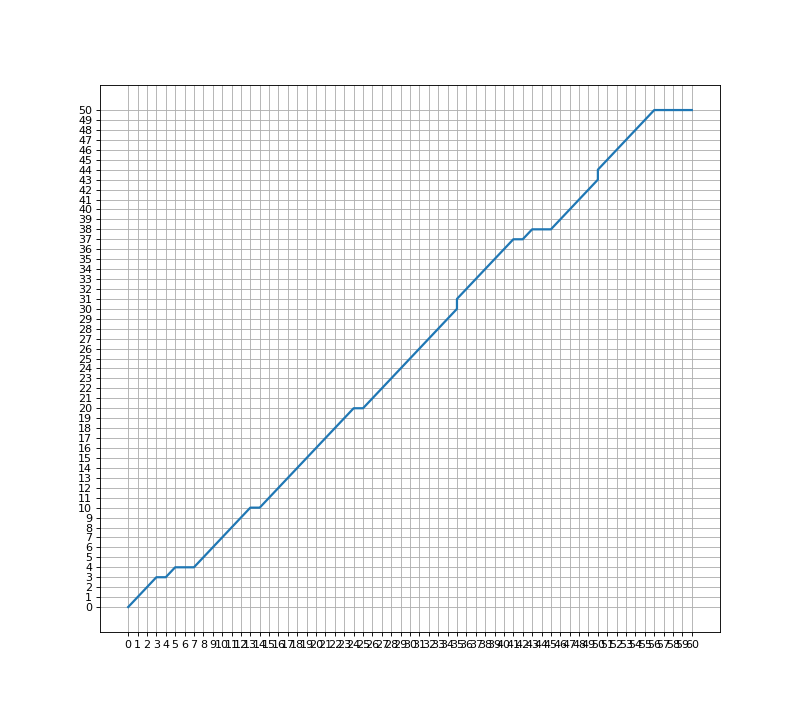
\includegraphics[width=1\textwidth]{figures/Figure_1.png}
        \caption{\textbf{Shortest Path}}\label{Test}
        \end{figure}
    \end{itemize}
    \end{solution}
\end{enumerate}

\vspace{20pt}

\textbf{Remark:} You need to include your .cpp, .pdf and .tex files in your uploaded .rar or .zip file.

%========================================================================
\end{document}
